\chapter{Trigger}



\section{Trigger Rates in High Luminosity Regime}
%\addcontentsline{toc}{section}{$e/\gamma$ Trigger authorship tasks}
The ATLAS trigger system comprises a
hardware-based Level-1 (L1) trigger and a software-based
High Level Trigger (HLT), subdivided into the Level-2
(L2) and Event Filter (EF). Due to the bandwidth
limitations of the trigger each level is restricted to a
certain output rate. During 2011 the L1 output rate was
kept below 60 kHz, L2 below 5 kHz and the EF output
rate at around 400 Hz averaged over the LHC fills. The
bandwidth allocated to the $e/\gamma$ triggers was
approximately 30\% of the total EF output rate.
Electron and photon identification is accomplished by a
set of $\eta$- and $E_{T}$-dependent rectangular cuts variables
\cite{trig1, trig2}.\\
Throughout 2011 data taking at ATLAS the luminosity continued to increase putting pressure on the trigger's ability to control the output rate. Several methods were employed to reduce the trigger rate and in the $e/\gamma$ trigger a variable threshold and hadronic core isolation was investigated to reduce the rate of the Level-1 trigger. In order to keep within time constraints only a coarse granularity is available Level-1 trigger in regions of 0.4 $\eta$. Threshold requirements were therefore investigated varying every 0.4 $\eta$. The effect of a hadronic core isolation was also investigated on the selection of electrons which defines a region in the hadronic calorimeter behind the $e/\gamma$ candidate in which you require and minimum amount of energy to be deposited to distinguish between jets and $e/\gamma$ objects. 


\begin{figure}[h!]
\centering
%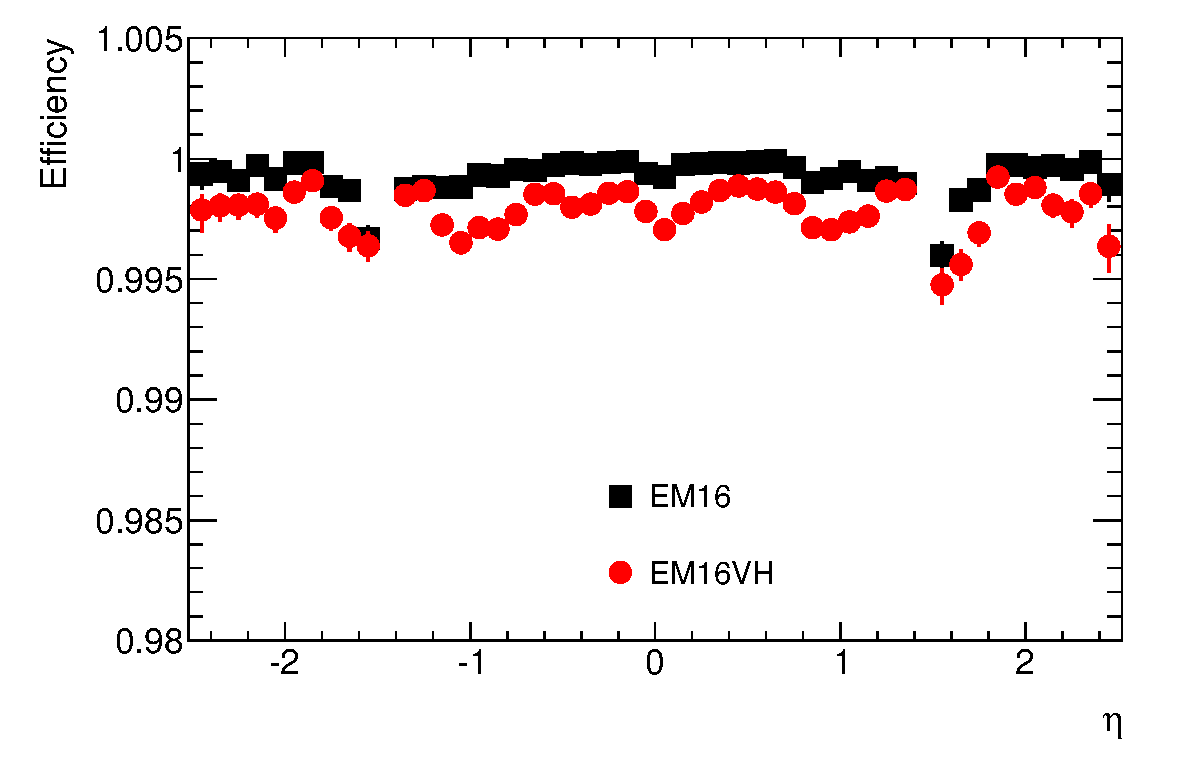
\includegraphics[width=0.49\linewidth]{images/L1_EM16VH_TandP_eff_vs_eta-eps-converted-to.pdf}
%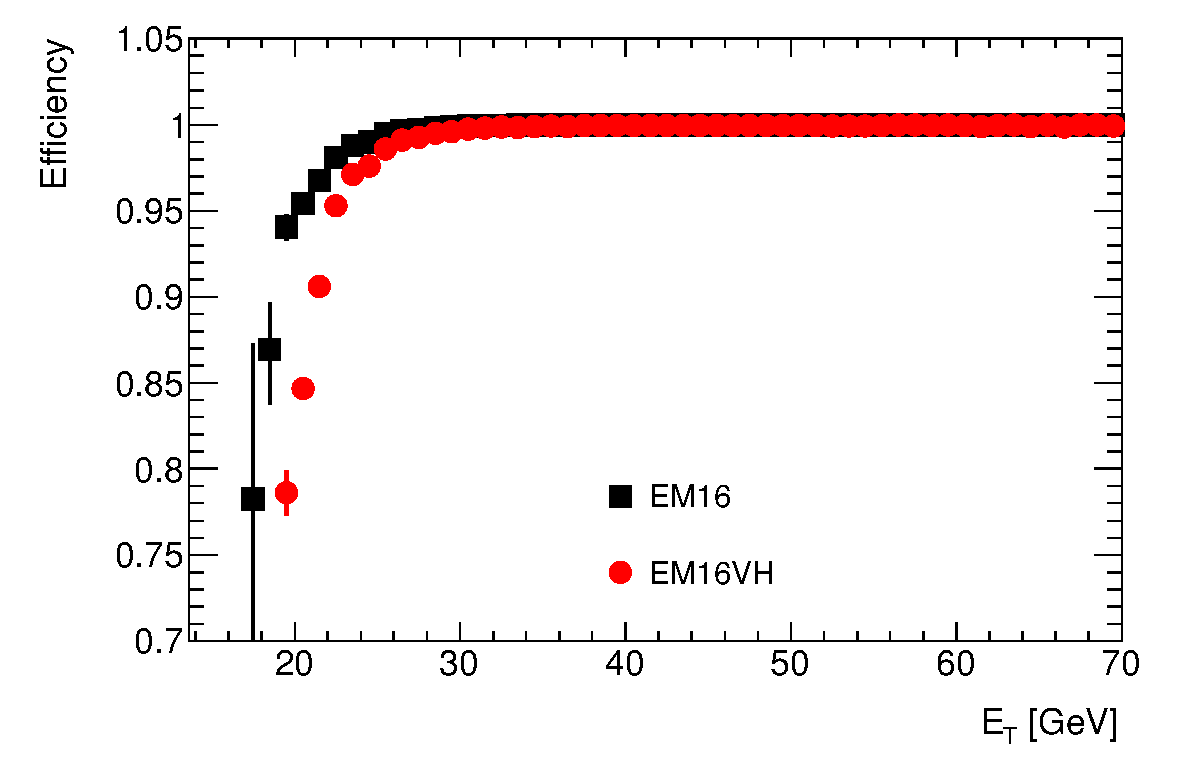
\includegraphics[width=0.49\linewidth]{images/L1_EM16VH_TandP_eff_vs_Et-eps-converted-to.pdf}

%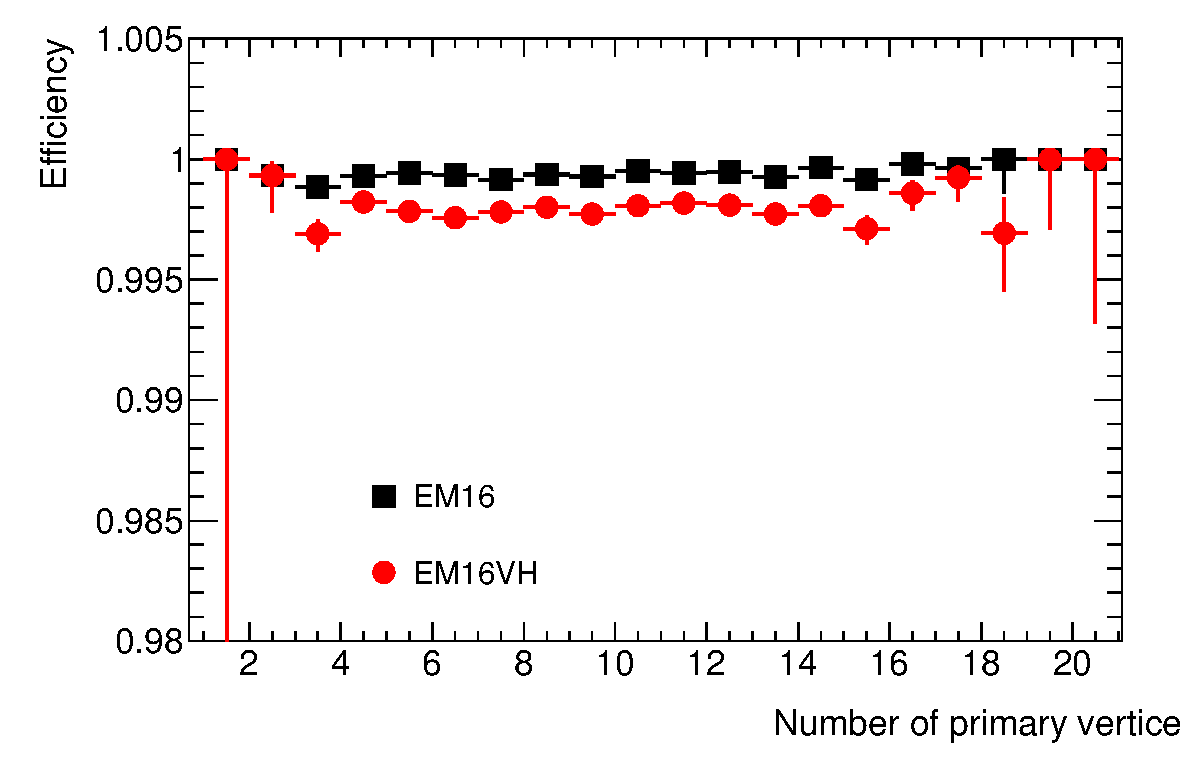
\includegraphics[width=0.49\linewidth]{images/L1_EM16VH_TandP_eff_vs_pvx-eps-converted-to.pdf}
\caption{Performance of the first level of the ATLAS $e/\gamma$ trigger before(EM16) and after(EM16VH) variable thresholds and hadronic core isolation are applied.}
\label{fig:L1}
\end{figure}

These attempts where successful and rate reduced to compensate for the high luminosity environment. Fig. \ref{fig:L1} shows the performance of the trigger after these changes had been made. It can be seen that a minimal impact of these new requirements is felt.


There was also a contribution to the maintenance of the $e/\gamma$ trigger software run in the ATLAS detector, both these tasks forming the authorship qualification. The authorship task culminated in presentation of a poster on behalf of the $e/\gamma$ trigger group at the Computing and High Energy Physics (CHEP) conference held New York in May 2012. The contribution is included two pages previously and details the performance of the $e/\gamma$ trigger in the 2011 run period \cite{poster}.

